%% IMPORTANT: Once working, run latex 3 times to get listoffigures to work

%% Be sure to check spelling!

%% Put **your** name and the proper due date in place

%% Note put your own file names in the appendix
%% Copy the relevant code as many times as needed for all files

%% Note that the \epsfig command is currently commented out

\documentclass{article}
\usepackage{amsmath}    % load AMS-Math package
\usepackage{epsfig}     % allows PostScript files
\usepackage{listings}   % allows lstlisting environment
\usepackage{moreverb}   % allows listinginput environment
\usepackage{vmargin}    % allows better margins
\setpapersize{USletter} % sets the paper size
\setmarginsrb{1in}{0.5in}{1in}{0.2in}{12pt}{11mm}{0pt}{11mm} %sets margins 
\begin{document}
\begin{center}
\rule{6.5in}{0.5mm}\\~\\
{\bf \large EGR 103L - Fall 2016}\\~\\
{\huge \bf Laboratory 7 - Linear Algebra}\\~\\
CEMAL YAGCIOGLU (cy111)\\
Lab Section 5D, Wednesday 11.45AM - 2.35PM\\
30 OCTOBER, 2016\\~\\
{\small  I understand and have adhered to all the tenets of the Duke
  Community Standard in completing every part of this assignment.  I
  understand that a violation of any part of the Standard on any part
  of this assignment can result in failure of this assignment, failure
  of this course, and/or suspension from Duke University.} 
\rule{6.5in}{0.5mm}\\
\end{center}
\tableofcontents
\listoffigures
\pagebreak
\section{Palm Problem 8.1}
\renewcommand{\arraystretch}{1.5}
\begin{center}
\begin{tabular}{|c||c|c|c|}\hline
Part & x & y & z \\ \hline \hline
$a$ & 2.4762e+00 & 2.4762e+00  & N/A\\ \hline
$b$ & -1.1818e+00 &  1.0909e+00 & N/A \\ \hline
$c$ & 3.0000e+00 & 5.0000e+00 & -2.0000e+00 \\ \hline
$d$ & 2.0035e+00 & -2.6848e+00  & 5.2312e+00 \\ \hline
\end{tabular}
\end{center}

\section{Based on Chapra Problem 8.3}
% Equations in matrix form
% Solutions for this system (x = vector)
% Transpose and inverse
% Condition numbers
% Meaning of condition numbers
\begin {align*}
\begin {bmatrix}{\mathbf A }\end{bmatrix}
\begin {Bmatrix}{\mathbf x }\end{Bmatrix}&=
\begin {Bmatrix}{\mathbf b }\end{Bmatrix}\\
\begin {bmatrix}
0 & -6 & 5 \\
0 & 2 & 7 \\
-4 & 3 & -7
\end {bmatrix}
\begin {Bmatrix}
~ x_1 ~ \\ x_2 \\ x_3
\end {Bmatrix}&=
\begin {Bmatrix}
50 \\ -30 \\ 50
\end {Bmatrix}
\end {align*}
Solution is:
\begin{align*}
\begin{Bmatrix}
-1.7019e+01 \\ -9.6154e+00 \\ 1.5385e+00
\end{Bmatrix}
\end{align*}
Transpose of the matrix A:
\begin{align*}
\begin{bmatrix}
0 & 0 & -4 \\
-6 & 2 & 3 \\
5 & 7 & -7 \\
\end{bmatrix}
\end{align*}
Inverse of the matrix A:
\begin{align*}
\begin{bmatrix}
-1.6827e-01 & -1.2981e-01 & -2.5000e-01 \\
-1.3462e-01 & 9.6154e-02 & 0 \\
3.8462e-02 & 1.1538e-01 & 0
\end{bmatrix}
\end{align*}
Condition number for 1 norm is 19. Condition number for 2 norm is 1.2062e+01. Condition number for Frobenius norm is 1.3711e+01. Condition number for infinity norm is 14. They show the relative error. Thus higher level norms can be said to give more reliable answers. 

\section{Based on Chapra Problem 8.10}
% Equations in matrix form
\begin{align*}
\begin{bmatrix}
-cos(30°) & 0 & cos(60°) & 0 & 0 & 0\\
-sin(30°) & 0 & -sin(60°) & 0 & 0 & 0\\
cos(30°) & 1 & 0 &2 & 0 & 0\\
sin(30°) & 0 & 0 & 0 & 2 & 0\\
0 & -1 & cos(60°) & 0 & 0 & 0\\
0 & 0 & sin(60°) & 0 & 0 & 2
\end{bmatrix}
\begin{Bmatrix}
F_1 \\ F_2 \\ F_3 \\ H_2 \\ V_2 \\ V_3
\end{Bmatrix}&=
\begin{Bmatrix}
~ 0 ~ \\ 2000 \\ 0 \\ 0 \\ 0 \\ 0
\end{Bmatrix}
\end{align*}

% Sentence introducing the following results: 
Answers of the Matrix:
\begin{center}
{\tt
\input{TrussData.txt}
}
\end{center}

\section{Palm 8.5(b)}
% Discussion of whether there is a c value with easily predicted solutions
When c is equal to zero, none of the other x,y,z variables has coefficients leading to x=y=z=0. This point can also be seen on the graph. As we are including both ends of the limits, taking 201 points gives us less rounded points and it also gives us the answer for when c variable is zero. If 200 was used, the c=0 would not be tested.
% Discussion of why there are 201 points

\section{Based on Palm 8.9}
% Equations in matrix form
\begin {align*}
\begin {bmatrix}
3 & -1 & -1 & 0 \\
-1 & 2 & 0 & -1 \\
-1 & 0 & 2 & -1 \\
0 & -1 & -1 & 3 
\end {bmatrix}
\begin {Bmatrix}
~ T_1 ~ \\ T_2 \\ T_3 \\ T_4
\end {Bmatrix}&=
\begin {Bmatrix} 
T_a \\ 0 \\ 0 \\ T_b
\end {Bmatrix}
\end {align*}

% Sentence introducing the following results:
Temperature data for $T_a$=120 degree Celcius and $T_b$=20 degree Celcius:
\begin{center}
\input{TempData.txt}
\end{center}
\section{Based on Palm 8.16(a)}
% Sentence introducing the table of results
The a,b,c values for the first part of the question are respectively 6,-7,5.Calculated coefficients of for the set of points are in the table below.

% Table of results.
\begin{center}
\begin{tabular}{|c|c|c|c|}
\hline
Points & a & b & c\\\hline
(1,4), (4, 73), (5, 120) & 6.00e+00 & -7.00e+00 & 5.00e+00\\
(1,4), (4, -73), (5, 120) & 5.47e+01 & -2.99e+02 & 2.48e+02\\
(1,4), (4, 73), (4, 120) & \bf{N/A} & \bf{N/A} & \bf{N/A}\\
(1,4), (4, 73), (5, -120) & -5.40e+01 & 2.93e+02 & -2.35e+02\\\hline
\end{tabular}
\end{center}

\pagebreak
\appendix
\section{Codes and Output}
% Put the name of your file in the subsection name 
% and the listinginput input
% Be sure to include the community standard in codes!
% Add \pagebreaks if they make sense
% Make as many copies as you need

\subsection{Problem Palm 8.1, p. 357}
\listinginput[1]{1}{Problem1.m}

\subsection{Problem Based on Chapra Problem 8.3, p. 226}
\listinginput[1]{1}{Problem2.m}


\subsection{Problem Chapra 8.10, pp. 226-227}
\listinginput[1]{1}{Problem3.m}


\subsection{Problem Palm 8.5(b), p. 359}
\listinginput[1]{1}{Problem4.m}

\subsection{Problem Based on Palm 8.9, p. 363-364}
\listinginput[1]{1}{Temperatures.m}


\subsection{Problem Based on Palm 8.16(a), pp. 367 a,b,c solver}
\listinginput[1]{1}{ABCSolver.m}


\subsection{Problem Based on Palm 8.16(a), pp. 367 Function}
\listinginput[1]{1}{findquad.m}


\pagebreak
\section{Figures}

\begin{figure}[htb!]
\begin{center}
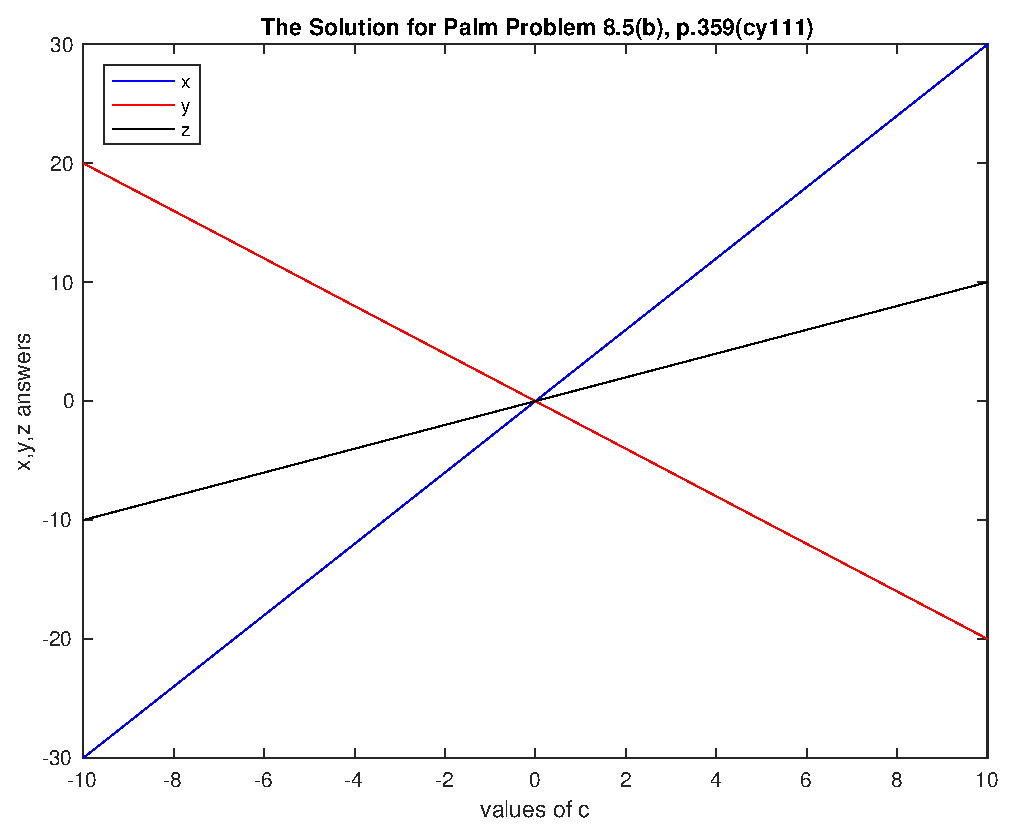
\epsfig{file=Problem4.eps, width=3.in}
\caption{Palm Problem 8.5(b), p.359}
\end{center}
\end{figure}


\begin{figure}[htb!]
\begin{center}
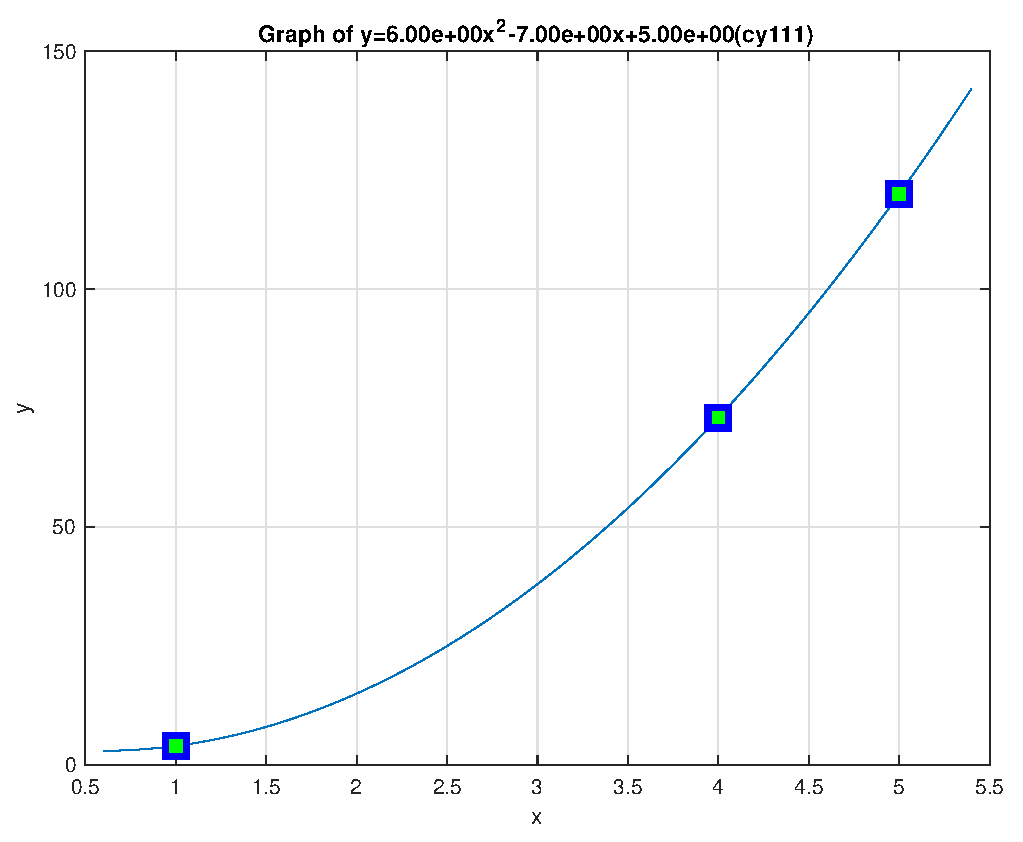
\epsfig{file=findquad1.eps, width=3.in}
\caption{Graph 1 for Palm 8.16(a), pp. 367}
\end{center}
\end{figure}


\begin{figure}[htb!]
\begin{center}
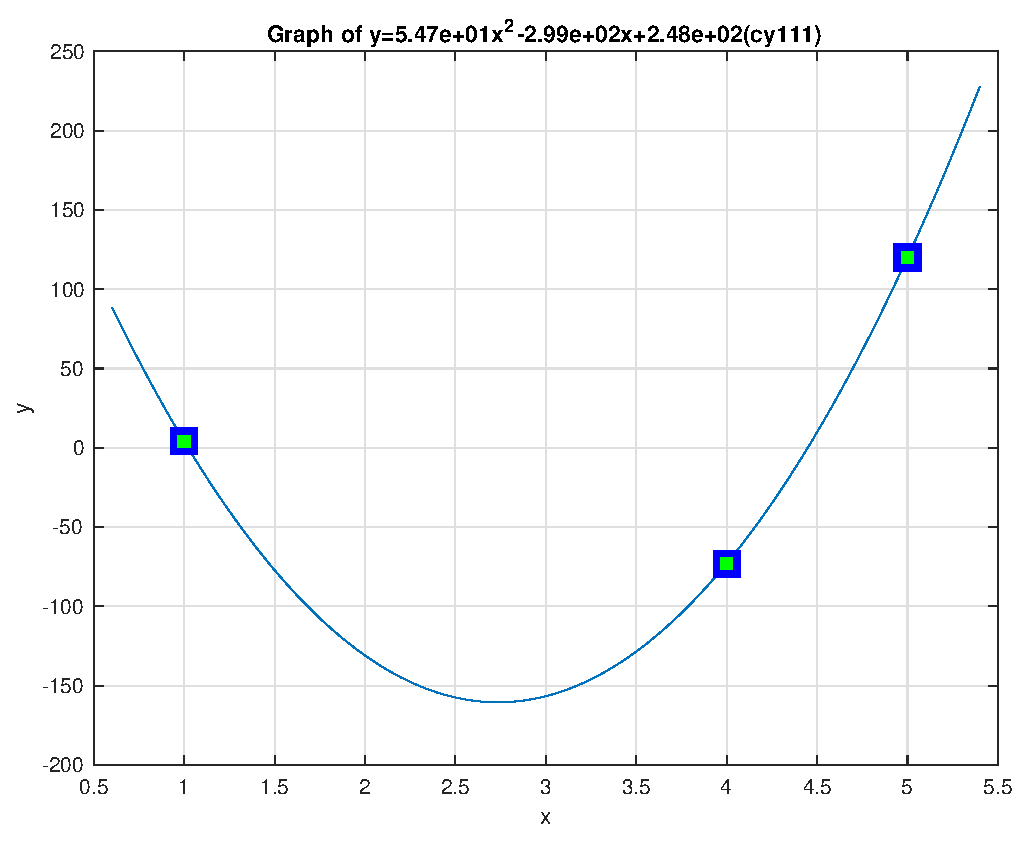
\epsfig{file=findquad2.eps, width=3.in}
\caption{Graph 2 for Palm 8.16(a), pp. 367}
\end{center}
\end{figure}


\begin{figure}[htb!]
\begin{center}
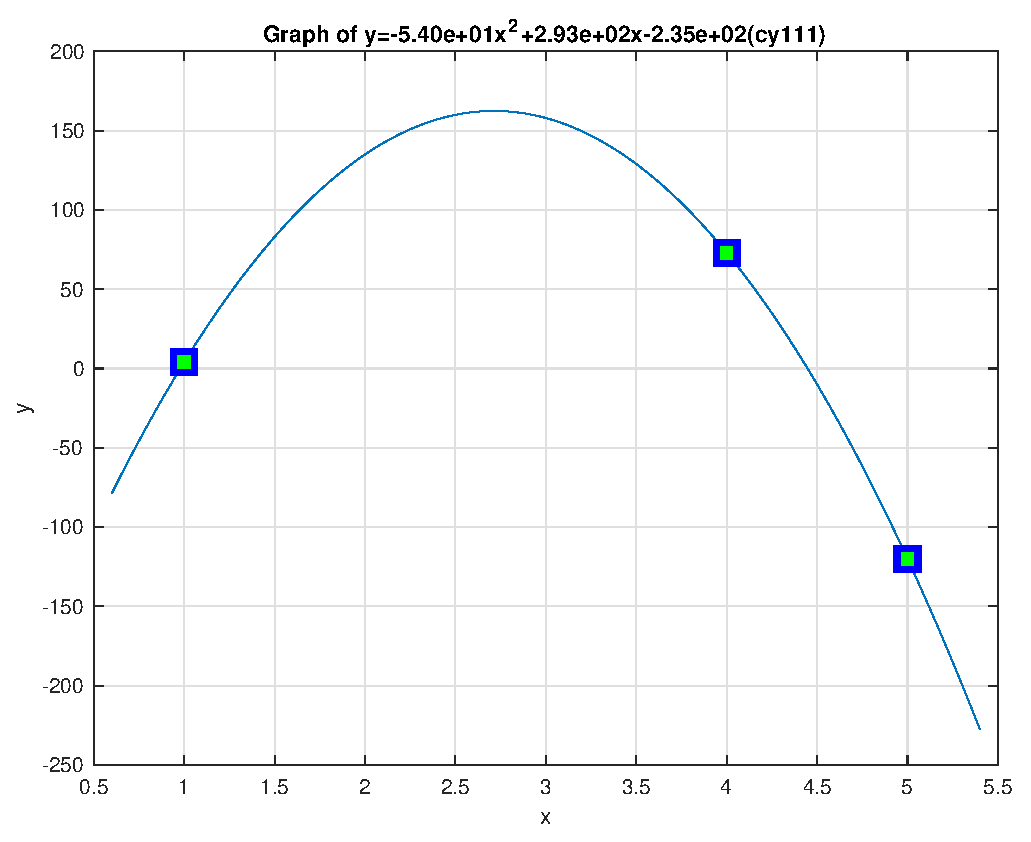
\epsfig{file=findquad3.eps, width=3.in}
\caption{Graph 3 for Palm 8.16(a), pp. 367}
\end{center}
\end{figure}

\clearpage
\begin{thebibliography}{9}
\bibitem{Chapra}
  Chapra, Steven C.,
  {\it Applied Numerical Methods with MATLAB for Engineering and Scientists}.
  McGraw-Hill, New York,
  3rd Edition,
  2012.
\bibitem{Palm}
  Palm, William J.,
  {\it Introduction to MATLAB for Engineers}.
  McGraw-Hill, New York,
  3rd Edition,
  2011.
\end{thebibliography}





\end{document}


